% Source page: original p. 308 (PDF p. 4)
% Figure number: Figure 1
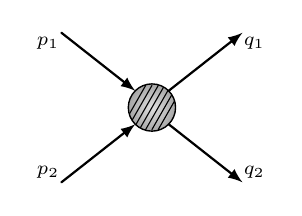
\begin{tikzpicture}[x=1cm,y=1cm,line cap=round,line join=round,>=latex]
  \def\r{0.30}
  \pgfmathsetmacro{\diag}{\r/sqrt(2)}

  \shade[inner color=black!12,outer color=black!35] (0,0) circle (\r);
  \draw[line width=0.5pt] (0,0) circle (\r);

  \begin{scope}
    \clip (0,0) circle (\r);
    \foreach \dx in {-0.24,-0.16,-0.08,0,0.08,0.16,0.24} {
      \draw[thin] (\dx-0.16,-0.28) -- (\dx+0.16,0.28);
    }
  \end{scope}

  \draw[->,line width=0.8pt] (-1.15,0.95) -- (-\diag,\diag);
  \draw[->,line width=0.8pt] (-1.15,-0.95) -- (-\diag,-\diag);
  \draw[->,line width=0.8pt] (\diag,\diag) -- (1.15,0.95);
  \draw[->,line width=0.8pt] (\diag,-\diag) -- (1.15,-0.95);

  \node[font=\scriptsize] at (-1.32,0.82) {$p_1$};
  \node[font=\scriptsize] at (-1.32,-0.82) {$p_2$};
  \node[font=\scriptsize] at (1.30,0.82) {$q_1$};
  \node[font=\scriptsize] at (1.30,-0.82) {$q_2$};
\end{tikzpicture}
